\documentclass[UTF8]{article}
\usepackage{ctex}
\usepackage{geometry}
\usepackage{cite}
\usepackage{tikz}
\usepackage{xcolor}
\usepackage{listings}
\usepackage{graphicx}
\usetikzlibrary{graphs, positioning, quotes, shapes.geometric}
\usepackage{url}
\usepackage{threeparttable}
%\usepackage{CJK}
\usepackage[colorlinks,
linkcolor=blue,
anchorcolor=blue, 
citecolor=blue,        
]{hyperref}
\usepackage{subfigure}
\usepackage[graphicx]{realboxes}
\usepackage{hyperref}
%\ctexset{bibname=}
\geometry{top=1cm}
\begin{document}
	\title{\vspace{+10pt} \heiti \textbf {基于孤立森林算法的智能水务分析模型}}
	\songti
	\author{oneboyi}
	\date{}
	\maketitle  
	\section*{\centering{摘要}}
		\par 如何通过有限的水流量数据来判断一个区域的供水系统是否发生故障是一个重要的问题,但是为了解决这个问题需要面对着许多挑战,比如模型的通用性、模型的性能、模型受噪声的影响等,
		可以说这些异常数据的检测至关重要,如何从大量水流量数据中快速找到异常数据是解决这些问题的关键所在。
		\par 论文从以上关键问题入手,首先,利用四分位距的方法,判断水流量数据的分布,水流量数据的分布不符合正态分布,因此不采用Z-score来判断异常数据,接着画出箱线图来具象化数据,可以找到数据的模式、水流量数据的特征,确立异常值的标准,初步找出超出范围之外的异常值,并把他们分为温和异常值和极端异常值。
		。但是箱线图只是能帮助初步分析数据,为了建立通用模型,文章接下来基于数据的特点进一步选取合适的算法,经过对数据模式的分析,抓住数据的特点,考虑了孤立森林算法,文章讨论了孤立森林算法是否适用于水流量数据的异常检测,并最终决定采用孤立森林算法来检测异常数据,后续的讨论中可以看到,孤立森林算法检测的异常值是符合上述异常值检测标准的。
		\par 文章分析了该方法的优缺点,孤立森林算法可以很好地快速处理大量数据,并且是一种无监督学习,鲁棒性好,可以很好地应对噪声地问题,即使没有异常数据也能够进行训练,但是如果异常数据差别不大或者异常数据太多,效果就会不明显。
		此外,该模型的优劣,取决于训练集的划分和参数的选取。可以通过箱线图对数据进行的分析来划分训练集,然后在测试集上进行测试,通过得到的结果来计算精确度等指标,评判该模型优劣并指出应该如何优化该模型。
		\\ \textbf{关键词: IQR、非正态分布、箱线图、孤立森林算法}
		\newpage
	\section{问题重述}
		\subsection{问题背景}
		\par 供水系统在我们的日程生活中至关重要,但是供水系统有时会发生各种各样的故障,从而导致漏水的发生,这是一个大问题。在这样的背景下,电磁流量计应运而生,用于测量流量以及监测漏水,一种方法是获取某一区域输入和输出水流量的插值加以评价。 
		\par 如今已经有许多基于流量数据的分析方法,但是还有一些挑战存在,比较重要的三个:首先是需要设计一个通用模型来了解流量计的数据模式,然后是如何更加快速地检测流量异常,最后一个挑战是如何应对噪声的影响。\cite[C1]{znswxxh}
		\subsection{具体问题}
		\par 您的团队需要设计一个模型来应对上述挑战,需要对给定数据进行清理,开发异常检测模型,并优化模型,数据是八个不同虚拟区域的输入水流量和输出水流量之差。具体的任务有:

		\begin{itemize}
			\item 分析数据模式,建立检测异常的标准
			\item 建立通用模型对八个区域进行异常值检测
			\item 测试模型并解释建模和异常值检测的结果
		\end{itemize}
		解决这些问题的关键是找到一个合适的异常数据检测算法。
	\section{数据模式分析与异常检测标准的确立}	
		\subsection{数据概览分析}
			\par 题目所给的数据来自于八个不同的虚拟地区,每个地区的流量差值是一个与时间相关的变量,这些值中既有正数,也有负数。大部分流量之差的绝对值都在10以内,如果发现绝对值过大,则可初步认为该数据是异常数据。流量数据随着时间的变化而变化,不同地区流量数据随时间变化的规律也各不相同。
			\par 首先判断各个地区的数据是否满足正态分布,采用四分位距的方法判断是否满足或者接近于正太分布,如果符合正态分布,则可以使用Z-score判断数据是否异常,如果不符合,则需要考虑其他的方法。
			\par 计算可得八个虚拟地区输入和输出水流量之差的四分位距:
			\begin{table}[!ht]
				\centering
				\resizebox{0.8\textwidth}{!}
				{
					\begin{tabular}{|l|l|l|l|l|l|l|l|l|}
					\hline
						region\_1 & region\_2 & region\_3 & region\_4 & region\_5 & region\_6 & region\_7 & region\_8 \\ \hline
						3.802019768 & 1.108408668 & 1.2881612 & 0.678413944 & 4.157332959 & 4.746437346 & 6.514955518 & 1.616935081 \\ \hline
					\end{tabular}
				}
			\end{table}
			\\可见并不满足正态分布的要求,因此不能采用Z-score判断数据是否异常。对于不满足正态分布的数据,可以使用箱线图进行异常数据的检测。
		\subsection{利用箱线图进行数据分析并检测异常数据}
			下面是根据八个地区数据所作出的箱线图\ref{Box},可以初步比较直观地对数据进行分析,也可以看出哪些是异常数据:
			\begin{figure}[!h]
				\centering %表示居中
				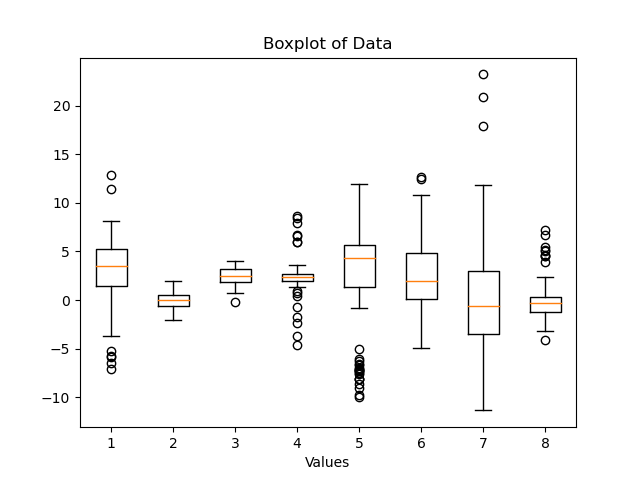
\includegraphics[height=4.5cm,width=9.5cm]{pictures/BoxPlot.png}
				% [height=4.5cm]表示高度
				%[width=9.5cm]表示宽度
				%{111.eps}表示eps格式的图片,名为111
				\caption{八个虚拟地区的箱线图}
				%图片的名称
				\label{Box}
				%图片的标签,用于文章中的引用,注意到标签的数字与实际文章显示的数字可能不同
			\end{figure}
			\par 从箱线图中,我们可以直观地看出每个地区的中位数、四分位数、异常数据以及数据的集中程度,箱线图较短的区域如2、3、4、8号地区数据集中程度就比较好。
			也可以用箱线图判断不同地区的数据趋向于哪种分布,比如区域三更趋向于正态分布,而其他区域的分布都有更多的偏移,既有左偏的分布又有右偏的分布,这些都可以直观地从箱线图中看出来。
		\subsection{异常检测的确立}
			已经使用了箱线图的办法,因此类似于正态分布中的3原则,可以借助第一、第三四分位数和四分位距IQR来对异常数据进行判断,对于每一个区域,
			找出他的第一和第三四分位数,然后先计算IQR:
			$$
			IQR=Q_3-Q_1
			$$
			然后计算内限范围:
			$$
			R_1=\left[ Q_1-1.5IQR,Q_3+1.5IQR \right] 
			$$
			以及外限范围:
			$$
			R_2=\left[ Q_1-3IQR,Q_3+3IQR \right] 
			$$
			处于内限范围以外的均为异常值,其中在外限以内的是温和异常值,在外限以外的是极端异常值。第4、5、8区域的异常值较多,第4区域的异常值最多,可以推测该地区的水流计发生了故障。
	\section{建立通用异常检测模型}
		\subsection{通用模型算法的选取}
			\par 通过箱线图进行分析以后,可以初步分析数据特征、找出异常数据,但是为了建立通用模型来检测异常数据,箱线图显然并不合适,箱线图只适合于反映数据的一些基本特征。
			\par 通过上述的箱线图可知,除了第四个区域异常数据稍多,其他区域异常值的占比都很低,且异常数据和正常数据的差别较大。因此可以采用孤立森林算法建立通用模型来进行异常值的检测。
			\par 孤立森林算法不需要对数据的分布做出假设,也不需要预处理数据,即使没有异常数据也能进行训练,这种算法大大降低了噪声的影响,训练所得模型可以快速处理大量数据并准确检测异常值\cite[iForest]{liu2008isolation}
			\par 下面展示了二维高斯分布中应用该方法找出孤立数据\cite{wikiif}
			\begin{figure} [!h]
				\centering
				\subfigure[\label{normal}]{
					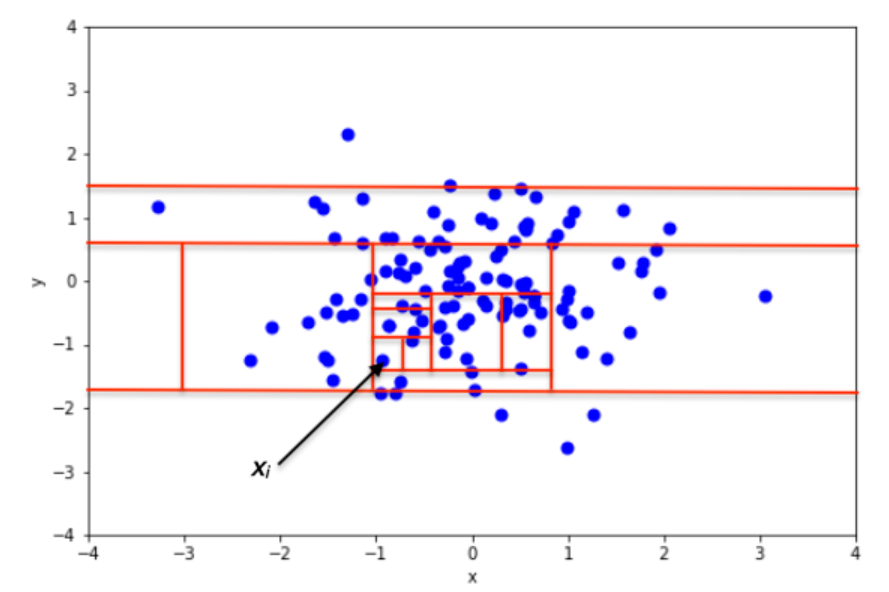
\includegraphics[scale=0.4]{pictures/iforest_example.png}}
				\subfigure[\label{abnormal}]{
					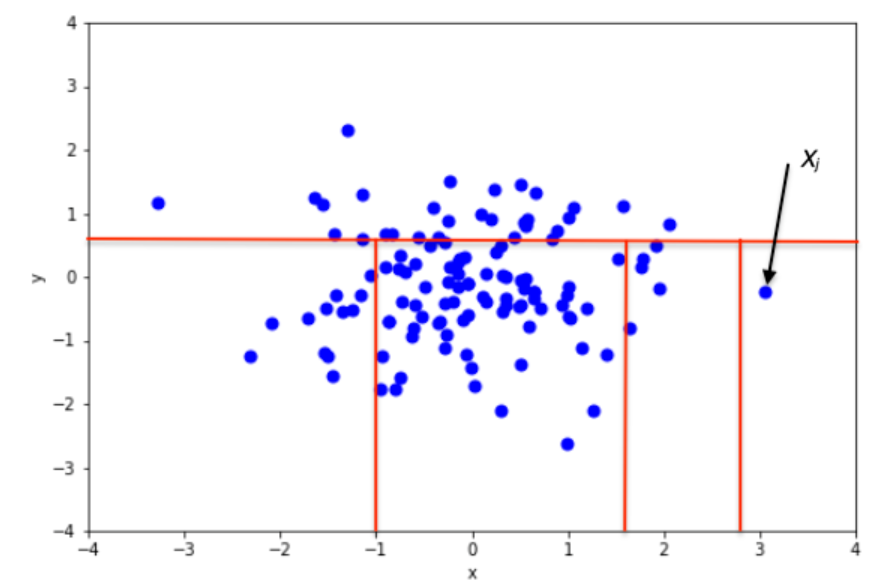
\includegraphics[scale=0.4]{pictures/wikiifi.png}}
				\caption{应用孤立森林算法的例子}
			\end{figure}
			\\图\ref{sub@normal}反映了正常数据的划分情形,而图\ref{sub@abnormal}反映了孤立点也就是异常数据的情形。
			\par 通过随机选择数据中的某些特征,并在这些特征的范围内随机选择一个划分点,将数据分配到树的不同分支上,直到每个叶子节点中只包含一个或少量的数据点。由于异常点很少,所以它们往往需要更少的分割才能被隔离到树的较深层。因此,异常点在孤立森林中的路径长度通常比正常点短。
			由于每个数据点都可以用路径长度来表示,因此可以将路径长度作为异常度量,即路径长度越小,则数据点越可能是异常值。
		\subsection{训练集的划分}
			\par 基于孤立森林法的特点,为了提高训练效果,提高模型的准确性、稳定性,应当选取异常数据较少地区的数据进行训练,另外,也要选取合适的参数。\cite{zhihuiif1}
	\section{模型的测试与评价}
	\bibliographystyle{unsrt}
	\bibliography{refs.bib}
	\section*{附录}
	\subsection*{I 程序源代码}
		hehe
	\subsection*{II 支撑材料文件列表}
	以下是建模过程中用到的文件
	\begin{itemize}
		\item 数据文件.xls:原始的数据文件
		\item sourcecode.rar:建模用到的代码文件以及运行代码所需的数据文件
	\end{itemize}
\end{document}